\documentclass{standalone}
\usepackage{tikz}
\usetikzlibrary{calc,patterns,decorations.pathmorphing,decorations.markings}

% node, begin anchor, end anchor, name
\newcommand{\makepoints}[3]{
    \foreach \k in {0, ..., \points}
    {
        \pgfmathsetmacro{\dist}{(\k-1) * (1 / (\points-1))}
        \coordinate (#1 \k) at ($(#2)!\dist!(#3)$);
    }
}

\begin{document}

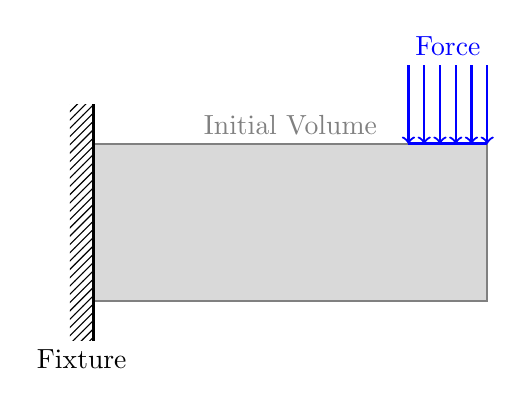
\begin{tikzpicture}[every node/.style={draw,outer sep=0pt,thick}]

% number of arrows between nodes
\pgfmathtruncatemacro{\points}{6}
        
\tikzstyle{ground}=[fill,pattern=north east lines,draw=none,minimum width=1cm,minimum height=0.3cm]


\node (M) [gray,label={[gray]Initial Volume},minimum width=5cm,minimum height=2cm,fill=gray!30] {};
\node (wall) at (M.west)[ground,label={west:Fixture},rotate=90,minimum width=3cm,yshift=0.15cm] {};
\draw[thick] (wall.south east) -- (wall.south west);
\node[draw=none] at (M.east){};

\coordinate (attackareaStart) at (M.north east);
\coordinate (attackareaEnd) at ($(attackareaStart)-(1,0)$);
\coordinate (forceStart) at ($(attackareaStart)+(0,1)$);
\coordinate (forceEnd) at ($(attackareaEnd)+(0,1)$);
\makepoints{bottom}{attackareaStart}{attackareaEnd}
\makepoints{top}{forceStart}{forceEnd}
% arrows
\foreach \i in {1, ..., \points} {
    \draw [->,blue,thick] (top \i) -- (bottom \i);
}
\draw[very thick,blue](attackareaStart)--(attackareaEnd);
\node[blue,above,draw=none](force) at ($.5*(forceStart)+.5*(forceEnd)$){Force};
\end{tikzpicture}

\end{document}